\documentclass[dvipdfmx]{jsarticle}
\usepackage[dvipdfmx]{graphicx}
\usepackage{HamadaLabThesis,comment,pxjahyper}


\lhead{\fancyplain{}{\rightmark}}
%
% 演習課題レポートの番号,氏名(学番号),提出日を明記すること.
%
\begin{document}
\title{\vspace{10zw}情報メディアプロジェクト I:最終課題レポート 1\\}
\date{\today} % 提出期限(厳守)
\author{\Large{\textbf{澤 \/ 祐里}}(21--1--037--0801)} % 氏名(学番号)
 
\thispagestyle{empty}
\maketitle
\thispagestyle{empty}
\clearpage

\pagenumbering{roman}
\setcounter{page}{1}
\setcounter{secnumdepth}{4}
\setcounter{tocdepth}{4}
\hypertarget{mokuji}{\tableofcontents}
\clearpage

\cfoot{\thepage \\ \hyperlink{mokuji}{目次へ}}
\pagenumbering{arabic}

\section{課題内容}
胃X線像6枚を用いて、健常胃と異常胃を分類するための方
法を提案し、実験結果(実行結果)を示す。更に、その
結果から提案手法を考察する。
\clearpage

\section{手順}
\subsection{課題1}
\subsubsection{計測対象}
\begin{itemize}
  \item 計測対象である画像処理は、画像のノイズを除去することができる「
  3×3メディアンフィルタを使った平滑化」である。
  この実験では、図\ref{graph:1}のようなプログラムを使う。
  \item 画像処理に用いる画像は、「幅512ピクセル × 高さ479ピクセル」の図\ref{graph:2}のような
  画像である。
  \begin{figure}[hbtp]
    \begin{minipage}[t]{\hsize}   
      \centering
      \caption{メディアンフィルタを使った平滑化のプログラム}
      \label{graph:1}
      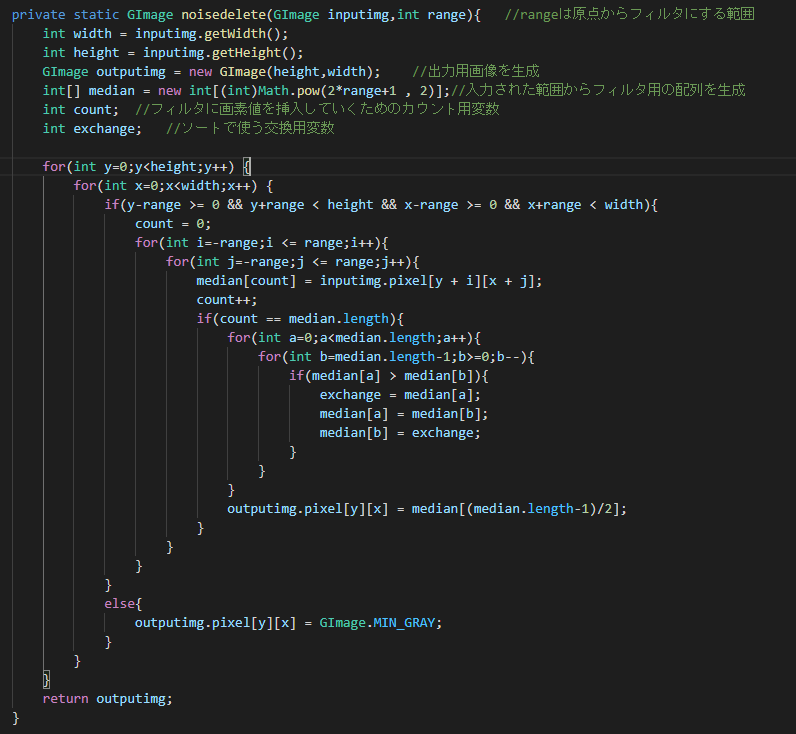
\includegraphics[scale = 0.75]{noisedeleteの中身1.PNG}
    \end{minipage}
    \begin{minipage}[t]{\hsize}
      \centering
      \caption{計測対象の画像処理に使う画像}
      \label{graph:2}
      \includegraphics[scale = 0.2]{d850429avhrr4.bmp}
    \end{minipage}
  \end{figure}
\end{itemize} 
\clearpage

\subsubsection{計測方法}
\begin{itemize}
  \item javaでは、「System.currentTimeMillis()」というメソッドを使うことで、long型で
  エポック秒から経過した時間をミリ秒単位で知ることができる。この実験では、
  このメソッドを用いて画像処理の処理時間を計測していく。
  \item 具体的な計測方法は「計測したい処理」を
  「System.currentTimeMillis()」で囲いこみ、処理後の時間から処理前の時間を引くことで
  、処理時間を計算する。
  \item 本題に入る前に、この計測方法が正確であるかどうかを
  確認する。javaの「Thread.sleep();」メソッドでは、引数に入れた数字×ミリ秒だけ、プログラムを
  一時停止することができる。これを利用して「Thread.sleep();」を処理とみなして、処理時間を
  計測し、「Thread.sleep();」の引数との比較を行うことで、計測方法が正確かどうかを判断する。
  \item この実験では、「Thread.sleep();」の引数を「1000」として、また、
  信頼性のあるデータをとるために、計測処理をfor文で20回繰り返えす図\ref{graph:5}のような
  プログラムを作成して計測した。その結果は、図\ref{graph:6}のようになり、結果をまとめると
  「1001ms」が9回、他は全て「1000ms」となった。1msの誤差が約1/2の確率で発生したが
  、この程度の誤差はマシンの性能などによる誤差の範疇だと考察できるため、
  この実験では、この計測方法は正確であると判断した。
  \item この実験では、画像処理の処理時間のみを正確に計測したいため、
  「System.currentTimeMillis()」を使って画像処理の処理時間を計測する前に、
  そもそもこの「System.currentTimeMillis()」という処理自体が時間を使っていないかを確認する。
  \item 計測方法は、図\ref{graph:3}のように、「System.currentTimeMillis()」を
  「System.currentTimeMillis()」で囲いこみ、処理後の時間から処理前の時間を引くことで
  、処理時間を計算する。また、信頼性のあるデータをとるために、これらの処理をfor文で
  20回繰り返している。
  \item 「System.currentTimeMillis()」の処理時間の計測結果は、図\ref{graph:4}の
  ように、試行回数20回の全てで「0ms」となった。これらの結果より、
  「System.currentTimeMillis()」の処理時間はこの実験では考慮しない。
  
  \begin{figure}[htbp]
    \begin{minipage}[t]{0.5\hsize}
      \centering
      \caption{「Thread.sleep();」を用いた計測方法の正確さ確認のプログラム}
      \label{graph:5}
      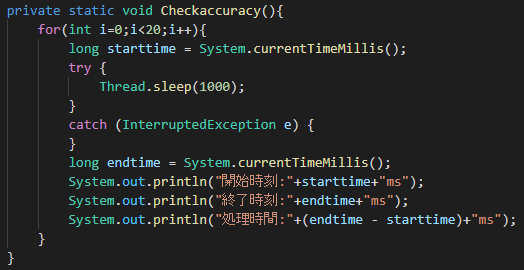
\includegraphics[scale=0.75]{計測方法の正確さを確認.PNG}
    \end{minipage}
    \begin{minipage}[t]{0.45\hsize}
      \centering
      \caption{「Thread.sleep();」を用いた計測方法の正確さ確認の出力結果}
      \label{graph:6}
      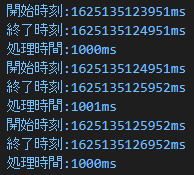
\includegraphics[scale=0.9]{計測方法の正確さを確認の出力.PNG}
    \end{minipage}
  \end{figure}
  \begin{figure}[htbp]
    \begin{minipage}[t]{0.5\hsize}
      \centering
      \caption{「System.currentTimeMillis()」の処理時間を計測するプログラム}
      \label{graph:3}
      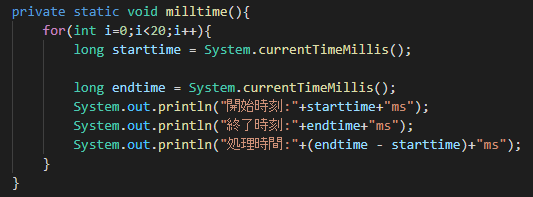
\includegraphics[scale=0.75]{milltimeのプログラム.PNG}
    \end{minipage}
    \begin{minipage}[t]{0.45\hsize}
      \centering
      \caption{「System.currentTimeMillis()」の処理時間の計測結果}
      \label{graph:4}
      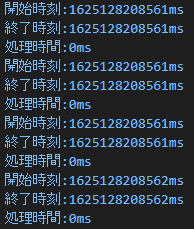
\includegraphics[scale=0.9]{milltimeの結果.PNG}
    \end{minipage}
  \end{figure}

\end{itemize}


\subsection{課題2}
\subsubsection{計測対象}
\subsubsection{計測方法}
\clearpage

\section{提案手法}
\begin{itemize}
  \item 前項の内容から、前処理は行わず、固定の画素値にとらわれずに異常胃を判別する方法を考える。
  \begin{itemize}
    \item[→] まず、健常胃の特徴は、画像を識別できるほどの特徴ではないと考え、
    異常胃のマスクメロン模様で判別しようと考えた。
    マスクメロン模様は異常胃の全ての画像に、びっしりと敷き詰められている。
    これを、異常胃には同じようなパーツが複数存在していると見立たてると、
    同じようなパーツが複数存在したら、異常胃であり、そうでなければ健常胃であると判別できると考えた。
    \begin{itemize}
      \item[→] そこで、私は3×3の配列を作成し、ある画素の周りを含めた9画素をその配列に格納し、中心の画素値と周りの
      8画素を比較する方法を考えた。この方法では具体的な画素値は必要とせず、比較を行うだけであるため、それぞれ画素値が違うマスクメロン模様の特徴を
      とらえることができると考えた。そのため、これを全画素に対して行い、比較の結果の合計を特徴量として、距離を計算し、ソートすることで異常胃を判別
      できると考えた。
    \end{itemize}
  \end{itemize}
\end{itemize}
以下に具体的な手順を示す。

\begin{enumerate}
  \item 図\ref{graph:1}のように、全画像の読み込みを行い、図\ref{graph:2}のインスタンスを作成。
  \item 画素値を入れるための3×3の配列を作成する。
  \item ある座標(x,y)の画素値と周りの座標(y-1,x-1)~(y+1,y+1)の画素値を配列に格納する。
  \item 図\ref{graph:3}のようにして、図\ref{graph:4}のような評価関数を呼び出し、中心の画素値と周りの画素値を比較する。
  \item (y-1,x-1)~(y+1,y+1)まで行い、中心の画素値より大きければ、配列pm[0]~pm[7]の値を1増やして、小さければ、配列pm[8]~pm[15]の値を1増やす。
  \item 上記の処理を端1画素を除いた全画素に行うまでループする。
  \item 配列pm[0]~pm[15]の値をその画像の特徴量として扱い、それぞれの画像と入力画像の特徴量の距離を図\ref{graph:5}のように求める。
  \item 距離が近い順に判別結果とする。
\end{enumerate}

\begin{figure}[htbp]
  \begin{minipage}[t]{0.45\hsize}
    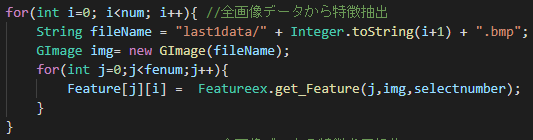
\includegraphics[scale=0.4]{画像読み込み.PNG}
    \centering
    \caption{画像読み込み}
    \label{graph:1}
  \end{minipage}
  \begin{minipage}[t]{0.25\hsize}
    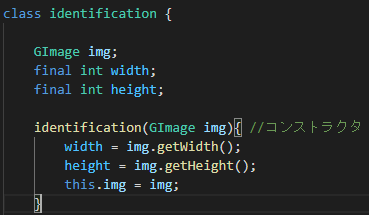
\includegraphics[scale=0.4]{クラス.PNG}
    \centering
    \caption{idenficationクラス}
    \label{graph:2}
  \end{minipage}
  \begin{minipage}[t]{0.25\hsize}
    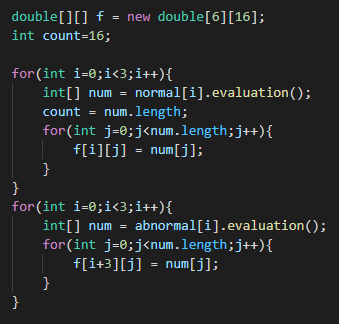
\includegraphics[scale=0.4]{評価関数呼び出し.PNG}
    \centering
    \caption{評価関数呼び出し}
    \label{graph:3}
  \end{minipage}
  \begin{minipage}[t]{0.45\hsize}
    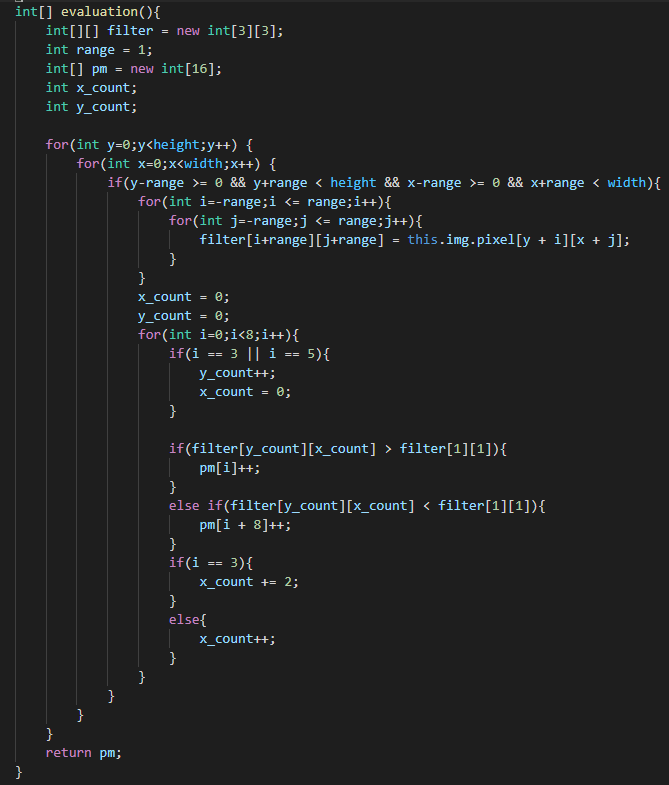
\includegraphics[scale=0.4]{評価関数.PNG}
    \centering
    \caption{評価関数}
    \label{graph:4}
  \end{minipage}
  \begin{minipage}[t]{0.45\hsize}
    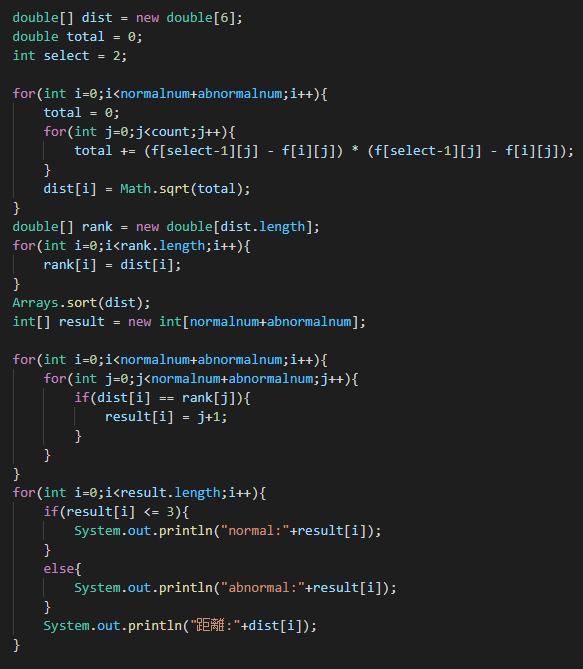
\includegraphics[scale=0.4]{距離計算.PNG}
    \centering
    \caption{距離計算とソート}
    \label{graph:5}
  \end{minipage}
\end{figure}

\clearpage

\section{考察}
\subsection{課題1}
\begin{itemize}
  \item 表\ref{table:1}と表\ref{table:6}を見ると、最初の2回分の処理時間が3回目以降の処理時間
  と比べて異常に長い。しかし、これらの処理は全て同じであり、本来は同じ処理時間が計測できる
  はずである。それに比べて、3回目以降は処理時間が安定しており、20回目以降も安定していると思われる。
  その中で、「Thread.sleep();」を使ったテストでは見られなかった「最初の2回だけ処理時間が長い」
  という現象は、ハードウェア的な問題であると考えられる
  。というのも、メディアンフィルタではソートなどを行うため、
  メソッドや配列などがあるメモリなどへのアクセスが頻繁に起こり、
  そういったアクセス時間が今回の計測結果の最初の2回分に影響したのではないかと考察した。
  また、3回目以降の計測時間が安定しているのは、最初の2回分の計測によるメモリへのアクセス過程で、
  メモリへのアクセスを高速化するパスのようなものが作成されていると考え、
  そのおかげであると考察した。
  \item 画像処理10回分、または画像処理20回分、繰り返してその回数で割った
  表\ref{table:2}と表\ref{table:3}の計測結果が1回分のデータと比べて
  、処理時間が短く安定しているように見えるのは、平均を取っているおかげであると考えられる。
  つまり、表\ref{table:2}と表\ref{table:3}でも、表\ref{table:1}と同様に、最初の2回分の
  処理時間が  異常に長くなっているが、その後の安定した「3回目以降の結果」で平均を取っているため、
  結果が安定しているように見えると思われる。実際に、表\ref{table:2}と表\ref{table:3}でも、
  1回目のデータは、他のデータに比べて「1,2ms」大きくなっている。
  しかし、こういった誤差は繰り返し回数を増やせば増やすほど、
  安定したデータが増えるために、減っていくと考察できる。
\end{itemize}

\subsection{課題2}
\begin{itemize}
  \item 表\ref{table:4}と表\ref{table:5}では、最終的な出力結果は同じで、違いはアルゴリズムだ
  けであるはずだが、処理時間は最初の2回だけなら、2倍弱も変わってしまっている。
  つまり、使うアルゴリズムによって処理時間は大きく変わるということになる。
  表\ref{table:4}で使ったバブルソートは、全てのデータを1つずつ比較してソートするアルゴリズムで
  あるため、メモリへのアクセス数は多いと考えられる。
  一方のクイックソートは、データを分けてソートするため、バブルソート
  よりはメモリへのアクセス数は少ないと考えられる。
  そのため、バブルソートを使ったプログラムよりもクイックソートを使ったプログラム
  の方が、処理時間が短くなったと考えられる。
\end{itemize}
\clearpage

\section{考察}

\begin{itemize}
  \item 表\ref{table:2}を見ると、検索結果1位と10位の検索キーとの距離が
  「0.415」と「1.694」となっており、約4倍も変わっていることが分かる。
  これは、検索に使う特徴ベクトルが8個もあるため、距離の計算の数値の振れ幅が大きくなった
  からであると考えられる。また、画像が100枚しか存在しないため、そもそもの類似画像が少なかった
  ことも原因であると考えられる。
  \item 検索結果の第3位、第4位、第5位を見比べてみる。
    \begin{itemize}
      \item 第3位の画像は四角形があり、その下に日本語が刻まれている。
      \item 第4位の画像は円形であり、その中にアルファベットが刻まれている。
      \item 第5位の画像は下向きの矢印が3本伸びている。
    \end{itemize}
    \begin{itemize}
      \item[→] このように、文字にしてみると第3位から第5位は全く別の画像のように聞こえるものの、
      検索キーとの距離を見ると、それぞれ「0.935」、「1.088」、「1.162」と
      なっており、距離は約0.1ずつほどしか変わっていないことが分かる。
      このような結果となった原因として、今回の課題で検索に使われた特徴は類似画像の
      検索に適していない、または、計算に使う特徴が足りていないということが考えられる。
      なぜなら、人間から見ると全く違う図形であるにも関わらず、距離が近いということは、
      「人間が画像を類似しているかどうかを判断している基準」をプログラムが
      計算に含めてきれていないと考えられるからである。
    \end{itemize}
    
\end{itemize}


\clearpage

\section{むすび}
今回の実験では、濃度、縦横比、水平ラン平均、垂直ラン平均、水平ラン標準偏差、垂直ラン標準偏差、重心x座標、
重心y座標の8つの特徴を用いて、キー画像の類似画像を検索するプログラムを作成した。
その結果として、それらの特徴がキー画像に近かったとしても、人間から見て類似画像であるとは限らないことが分かった。
今後、課題プログラムにおいて図形の検索精度を上げるためには、検索に使用する特徴の数を増やす
ことなどが挙げられる。


\clearpage

\begin{thebibliography}{9}
  \bibitem{url1} \url{https://www.javadrive.jp/start/stream/index4.html}
  \bibitem{url2} \url{https://www.javadrive.jp/start/scanner/index1.html}
\end{thebibliography}

\end{document}